\subsection{Results}
\label{Results}
\setlength{\parindent}{20pt}
\justifying

\subsubsection{\large{\emph{Participants}}}
\label{Exp1_ParticipantExclusion}

\noindent
After participant exclusions, 193 participants were retained in the final sample. Of these, 112 were male. Participants' mean age was 22.96 years.

\subsubsection{\large{\emph{Testing error}}}

\noindent
Unfortunately, due to a technical issue, the fifth round of training showed participants a single word, repeated eighty times. Due to this over-familiarisation, the word as well as its composing morphemes was excluded from all subsequent analyses.


\subsubsection{\large{\emph{Group-level analyses}}}

\noindent
\underline{Familiarity test}

\noindent
Participants significantly chose known morphemes above matched controls in an estimated 57\% of trials (t(192) = 9.16, p $<$ 2.2e$^{-16}$).

\begin{figure}[!htbp]
    \begin{center}
        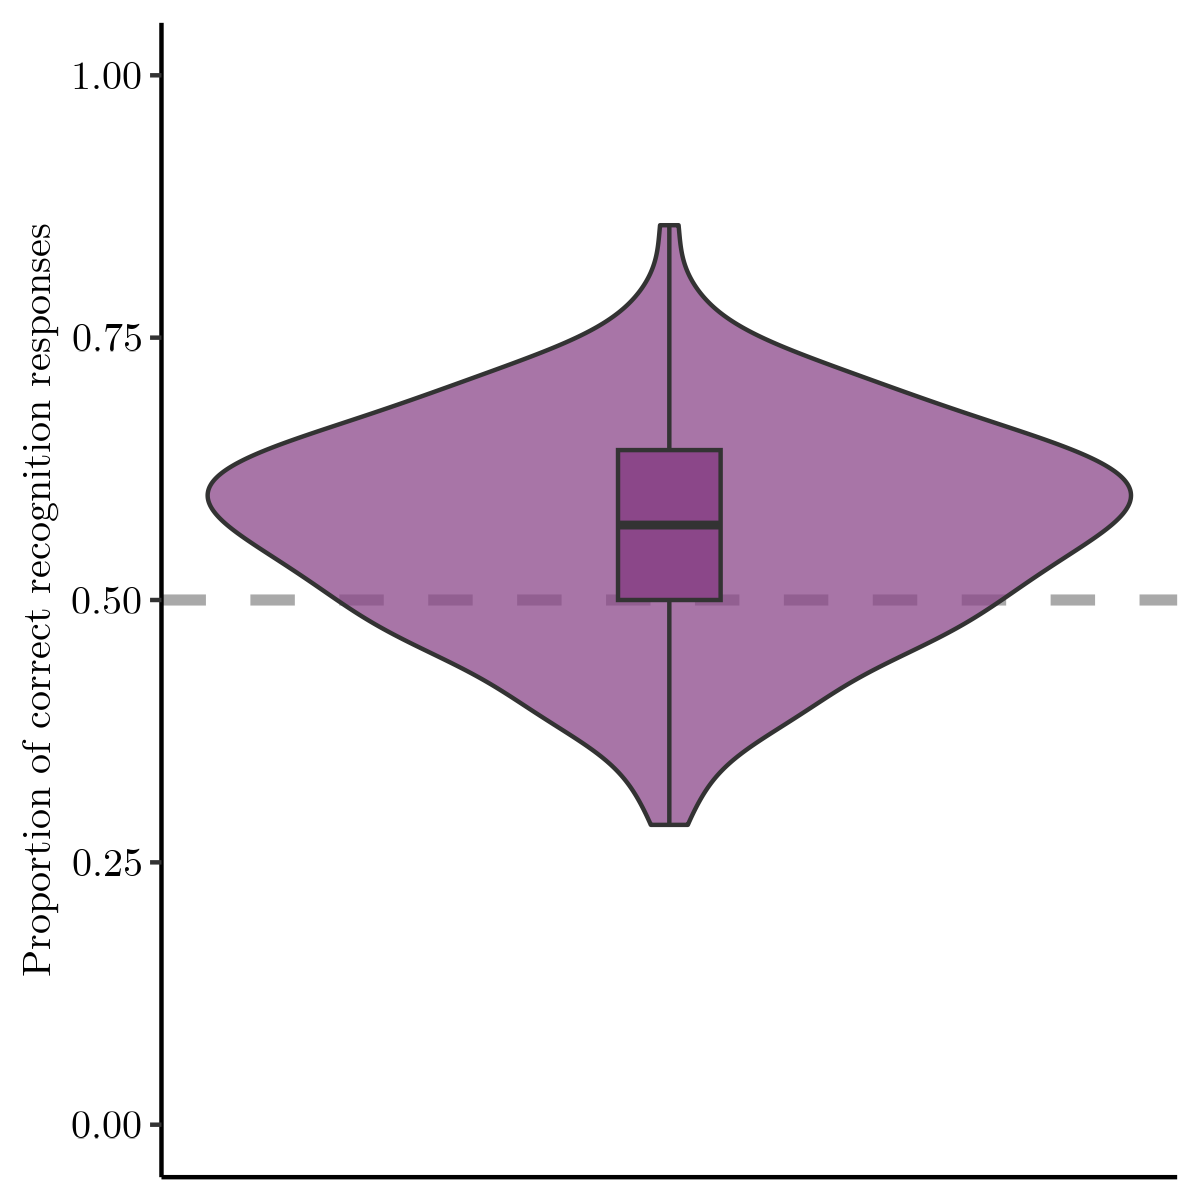
\includegraphics[width=0.6\textwidth]{Figures/exp1_familiarity_violinplt.png}
    \end{center}
    \caption[]{\justifying Violin plot and boxplot of the accuracy of familiarity test responses. The dashed line indicates chance level.}
    \label{exp1_familiarity}
\end{figure}

\noindent
\underline{Morpheme familiarity effect}

\noindent
Participants' responses across testing conditions is represented in \autoref{exp1_morphfam}. Linear modelling showed significant differences between each testing condition. The proportion of ``within-language'' responses in the 0M condition didn't significantly differ from chance (Intercept $\beta$ = -0.05, z = -1.06, p = 0.29). There were significantly more ``within-language'' responses in the 1M condition ($\beta$ = 0.28, z = 7.22, p = 5.31e$^{-13}$), and even more in the 2M condition ($\beta$ = 0.67, z = 12.74, p =3.402e$^{-37}$). Estimated marginal means analysis estimated the proportion of ``within-language'' responses to be 49\% for 0M , 56\% for 1M, and 65\% for 2M.

\begin{figure}[!htbp]
    \begin{center}
        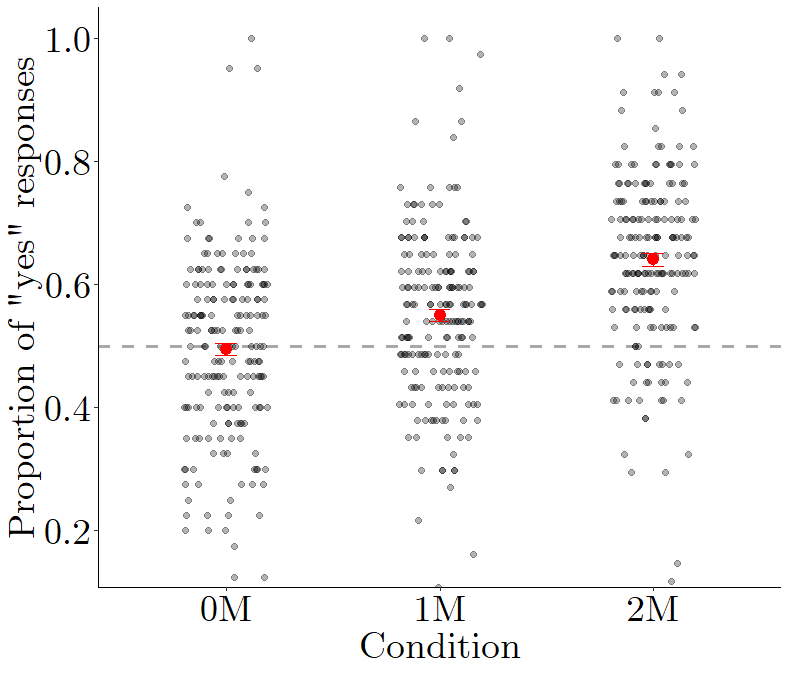
\includegraphics[width=0.6\textwidth]{Figures/Exp1_yes_allconditions.png}
    \end{center}
    \caption[]{\justifying Proportion of ``yes'' responses in each testing condition. The dashed line indicates chance level. The red circle shows the group mean, with bars as the standard error of the mean.}
    \label{exp1_morphfam}
\end{figure}

\noindent
\underline{2M performance}

\noindent
Overall, performance in the 2M condition was not significantly different from chance (t(192) = -0.64, p = 0.53). D-prime analysis yielded an average c of -0.37 (t(192) = -12.39, p$<$ 2e$^{-16}$) and average d-prime of -0.02 (t(192) = -0.76, p = 0.45): while participant responses were biased towards ``yes'', a d-prime so close to zero indicates no detection of the underlying structure. Response times and accuracy in the 2M condition were uncorrelated (r(191) = 0.04, p = 0.58), meaning there was no speed-accuracy trade-off here.

\begin{figure}[!htbp]
    \begin{center}
        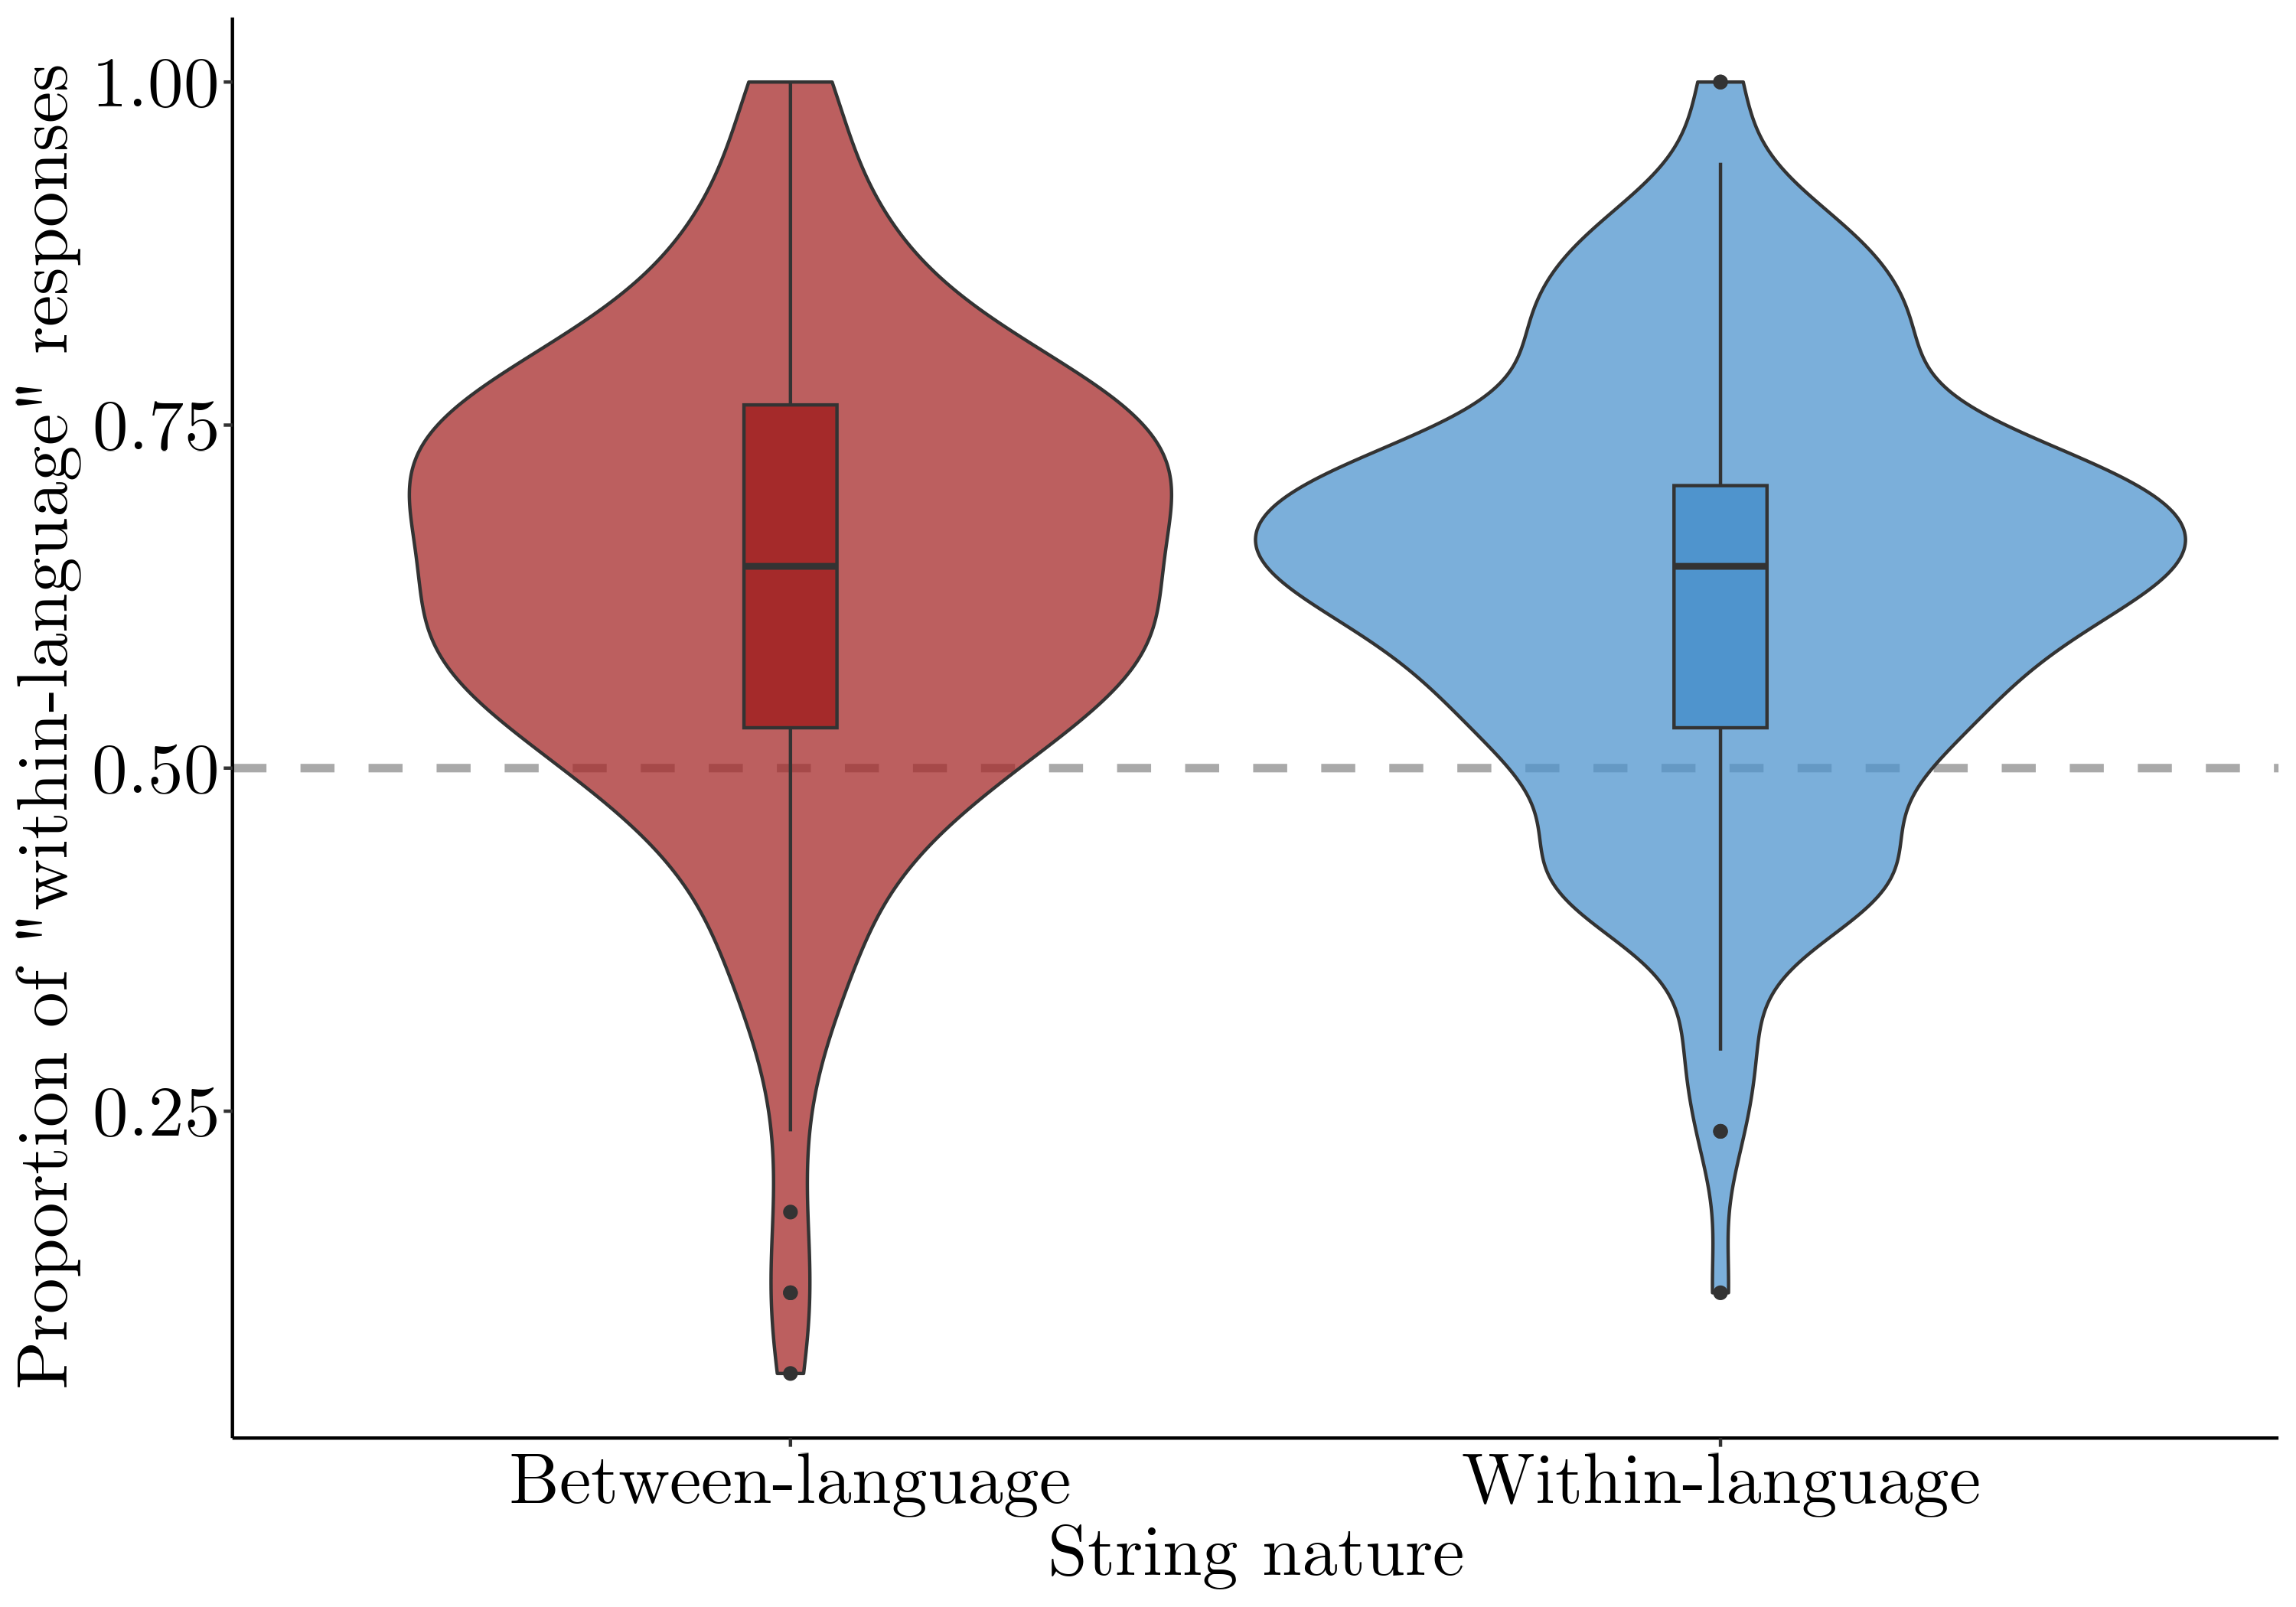
\includegraphics[width=0.6\textwidth]{Figures/exp1_2M_responses.png}
    \end{center}
    \caption[]{\justifying Boxplots of the proportion of ``within-language'' responses to each 2M combination type. The dashed line indicates chance level.}
    \label{exp1_2Mresponses}
\end{figure}

\subsubsection{\large{\emph{Individual differences analyses}}}

\noindent
\underline{BLP}

Lots of possible vars - after exp1 data, drop vars that are too similar so simplify down num of vars looked at

\noindent
In the BLP, 5 participants reported information on just one spoken language, 83 for two, 56 for three, and 49 for four. Of note is that the BLP instructions permitted reporting of languages spoken with any proficiency at all, so these divisions cannot be thought of as fluent monolingual/bilingual/trilingual/quadrilingual participants. The most popular L1 was Portuguese, the most popular L2 was English, the most popular L3 was Spanish, and the most popular L4 was French. Six unique language families were present in this sample, with a total of ten unique branches, and thirty-nine total languages. Out of these participants, 173 spoke languages with the same script, and 20 with different scripts. 

The Pearson correlation between entropy and multilingual experience scores indicated that these metrics are very strongly positively correlated: t(191) = 37.30, p $<$ 2e$^{-16}$, estimated r  = 0.94. On the other hand, the correlation between cosine similarity and multilingual experience shows these measures as distinct: t(191) = -1.68, p = 0.09, estimated r = -0.12. This provides evidence for the necessity of the cosine similarity measure as a multilingual metric separate from the influence of the number of languages contributing to its calculation.  

\noindent
\underline{PCA}

\noindent
The PCA extracted several PCs that will be used in subsequent analyses. PC1 was composed of L3 components, and makes up 17\% of the variance in scores. PC9 was the L4 equivalent, worth 13\% of variance. PC2 was of particular interest to the authors, as it strongly negatively weighs L1 use against strongly positively weighted L2 use (12\% of variance explained). PC8 loaded L2 history (how early participants speak a language well, 6\% of variance), while RC3 loaded L2 proficiency (6\% of variance). The resulting scree plot can be found in the \nameref{SuppMaterials}.

\noindent
\underline{Familiarity test}

\noindent
No variables significantly influenced familiarity responses. 

\noindent
\underline{Morpheme familiarity effect}

\noindent
There were significant interactions of all levels of multilingual category with the different testing conditions compared with the intercept (monolinguals). However, given the extremely low number of observations of monolinguals (n = 5), these effects were deemed unreliable. 

PC8 (L2 history) was significant as a main effect on ``yes'' responses ($\beta$ = 0.11, z = 2.38, p = 0.02), with longer L2 history prompting more ``yes'' responses. Earlier bilinguals might therefore be predisposed to accept a wider range of stimuli as linguistically-coherent. Older participants accepted fewer combinations overall ($\beta$ = -0.10, z = -2.21, p = 0.03), an effect seemingly driven by an increase in rejections of the 0M novel combinations. Indeed, the morpheme familiarity effect was stronger for older participants (Age*1M interaction: $\beta$ = 0.07, z = 1.92, p = 0.054; Age*2M interaction: $\beta$ = 0.14, z = 2.77, p = 0.006). Adults with more exposure to different language systems over the course of their life may be more reliant on previously seen chunks.

\begin{figure}[!htbp]
    \begin{center}
        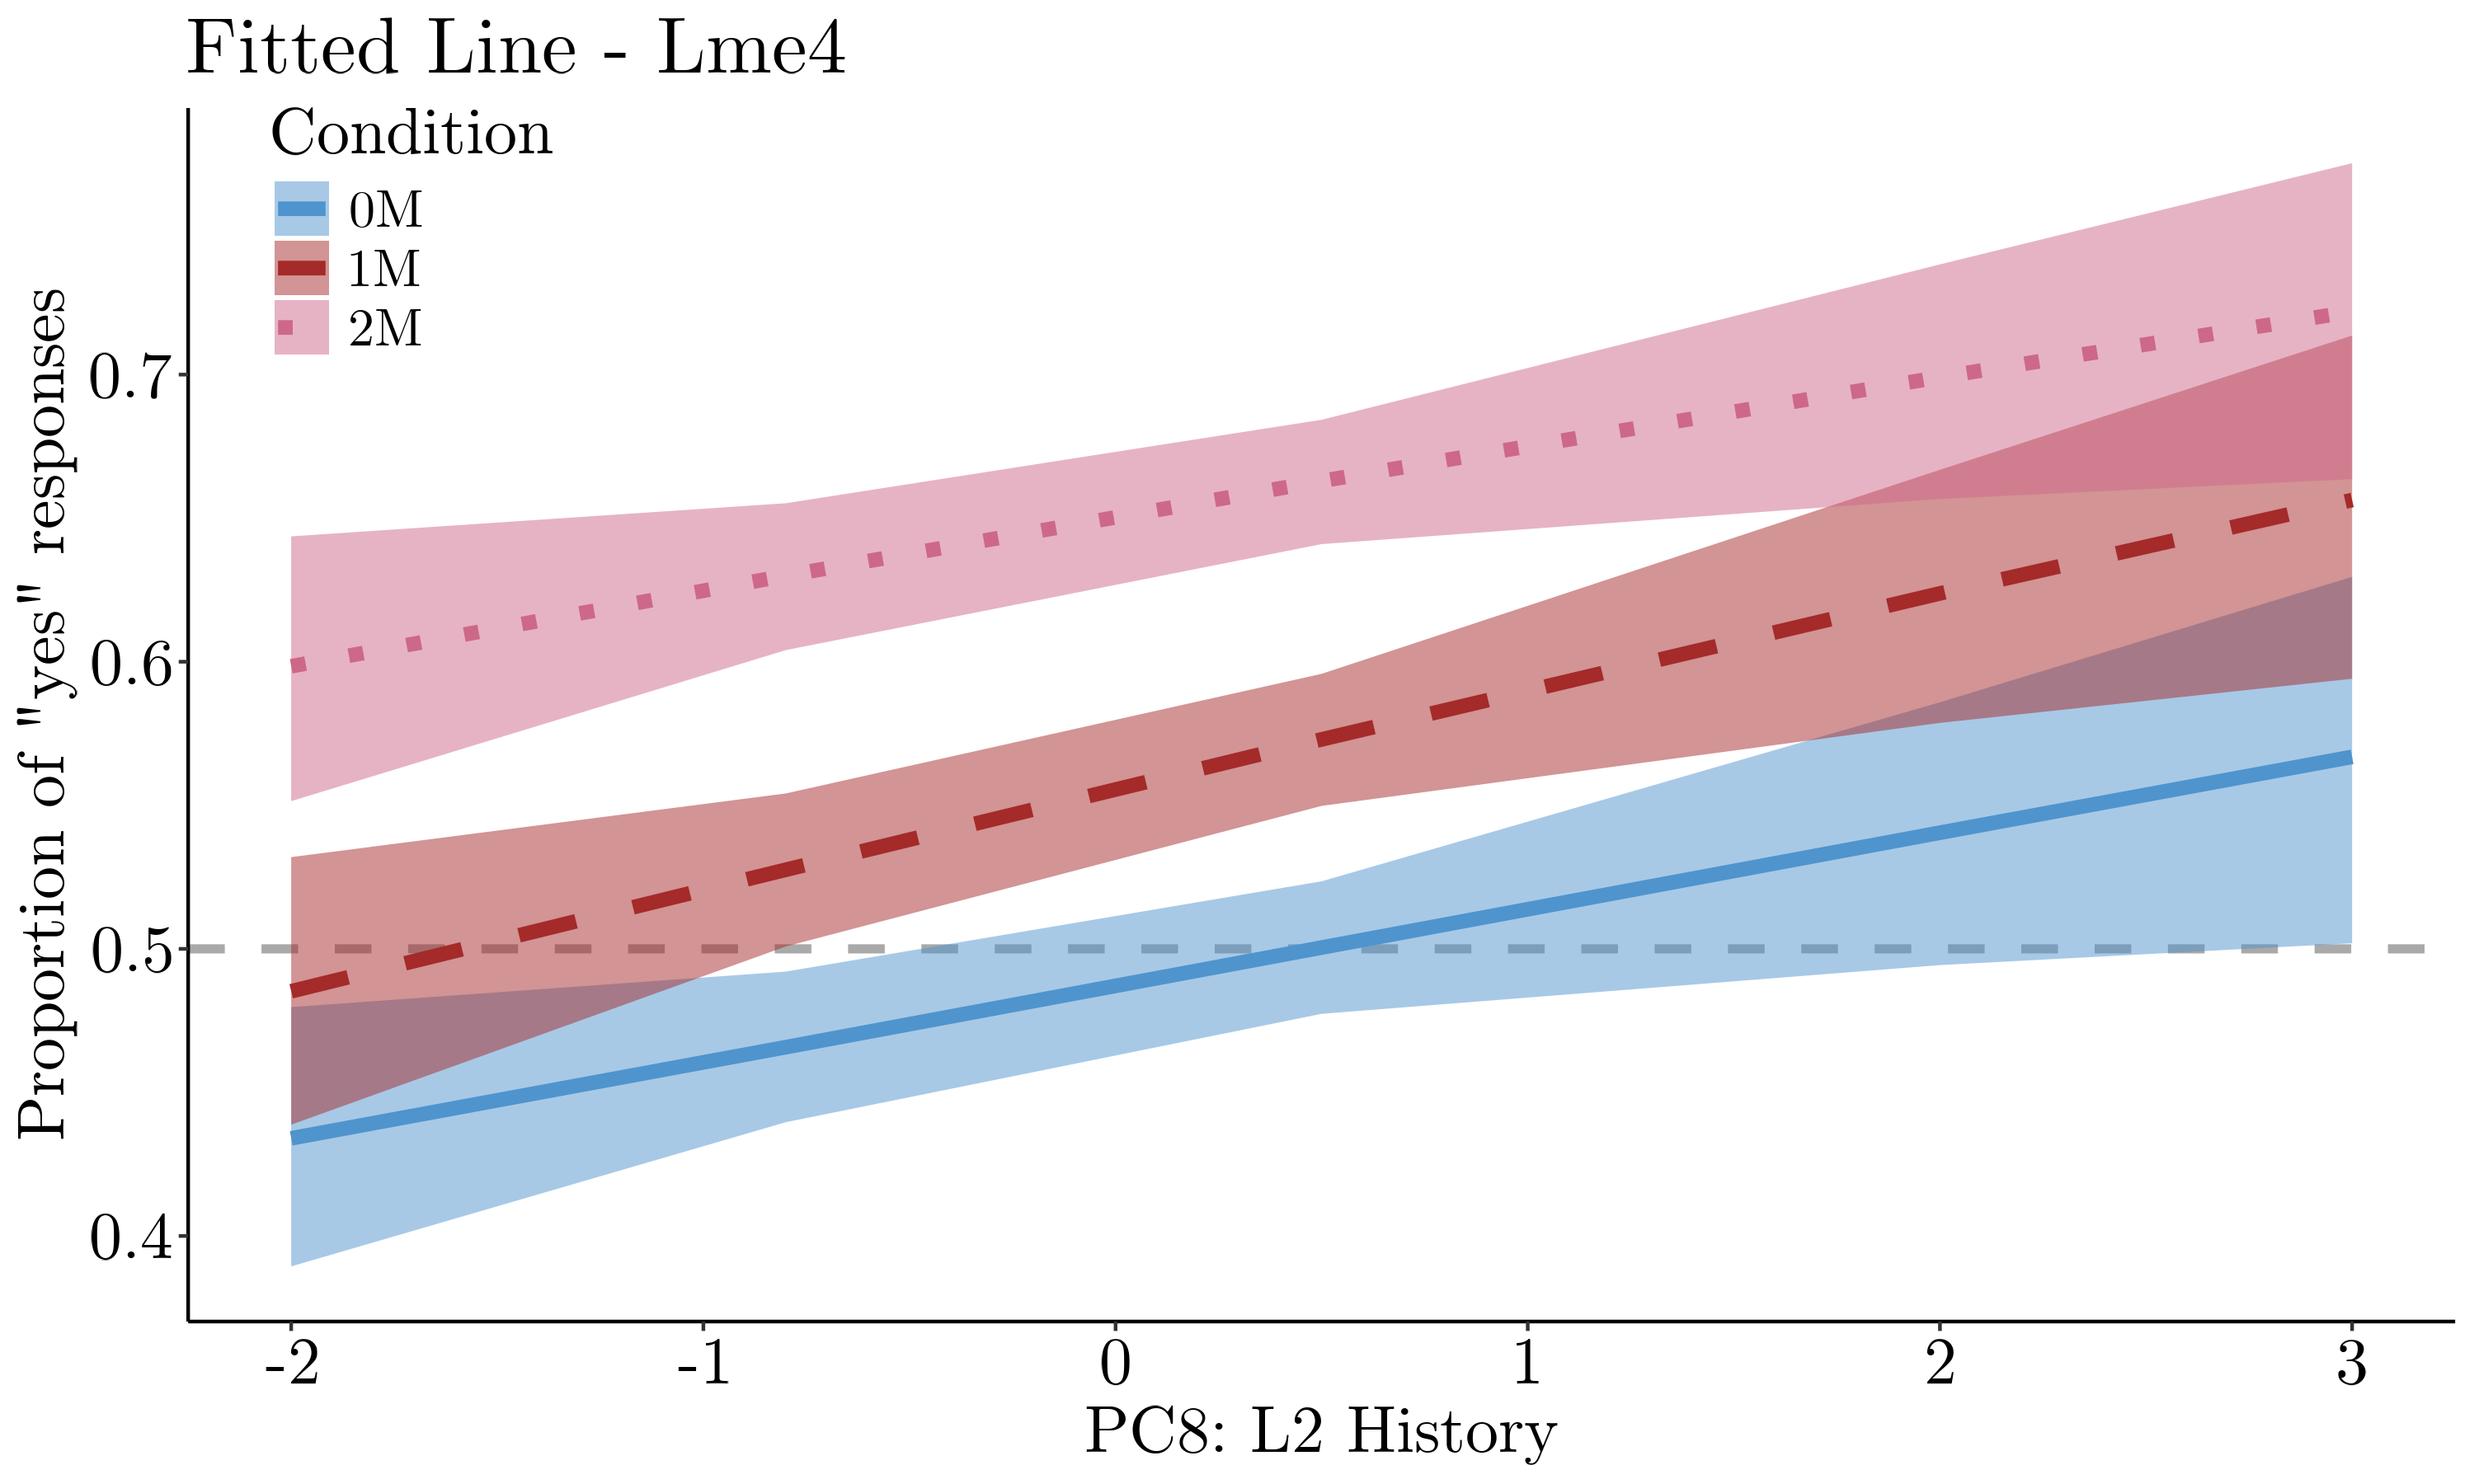
\includegraphics[width=0.6\textwidth]{Figures/Exp1_yes_PC8.png}
    \end{center}
    \caption[]{\justifying Model estimates of the effect of PC8 (L2 History) on ``yes'' responses, for the 0M (blue), 1M (red), and 2M conditions (pink). Higher values of PC8 translates to earlier experience and abilities in L2. Bars around the lines indicate the 95\% confidence interval. Dashed lines at 0.5 indicate chance level.}
    \label{exp1_yes/PC8}
\end{figure}

PC3 (L2 proficiency) also strengthened the morpheme familiarity effect (PC3*1M interaction: $\beta$ = 0.08, z = 2.24, p = 0.03; PC3*2M interaction: $\beta$ = 0.15, z = 2.91, p = 0.004). This was also the case for L1-L2 difference, which interacted significantly with the 1M and 2M conditions (L1-L2 difference*1M interaction: $\beta$ = -0.10, z = -2.81, p = 0.005; L1-L2 difference*2M interaction: $\beta$ = -0.13, z = -3.65, p = 0.0003). It may be that those with a more fluent and balanced interaction of their languages are better able to use past knowledge about new stimuli.

\begin{figure}[!htbp]
    \begin{minipage}{0.49\linewidth}
        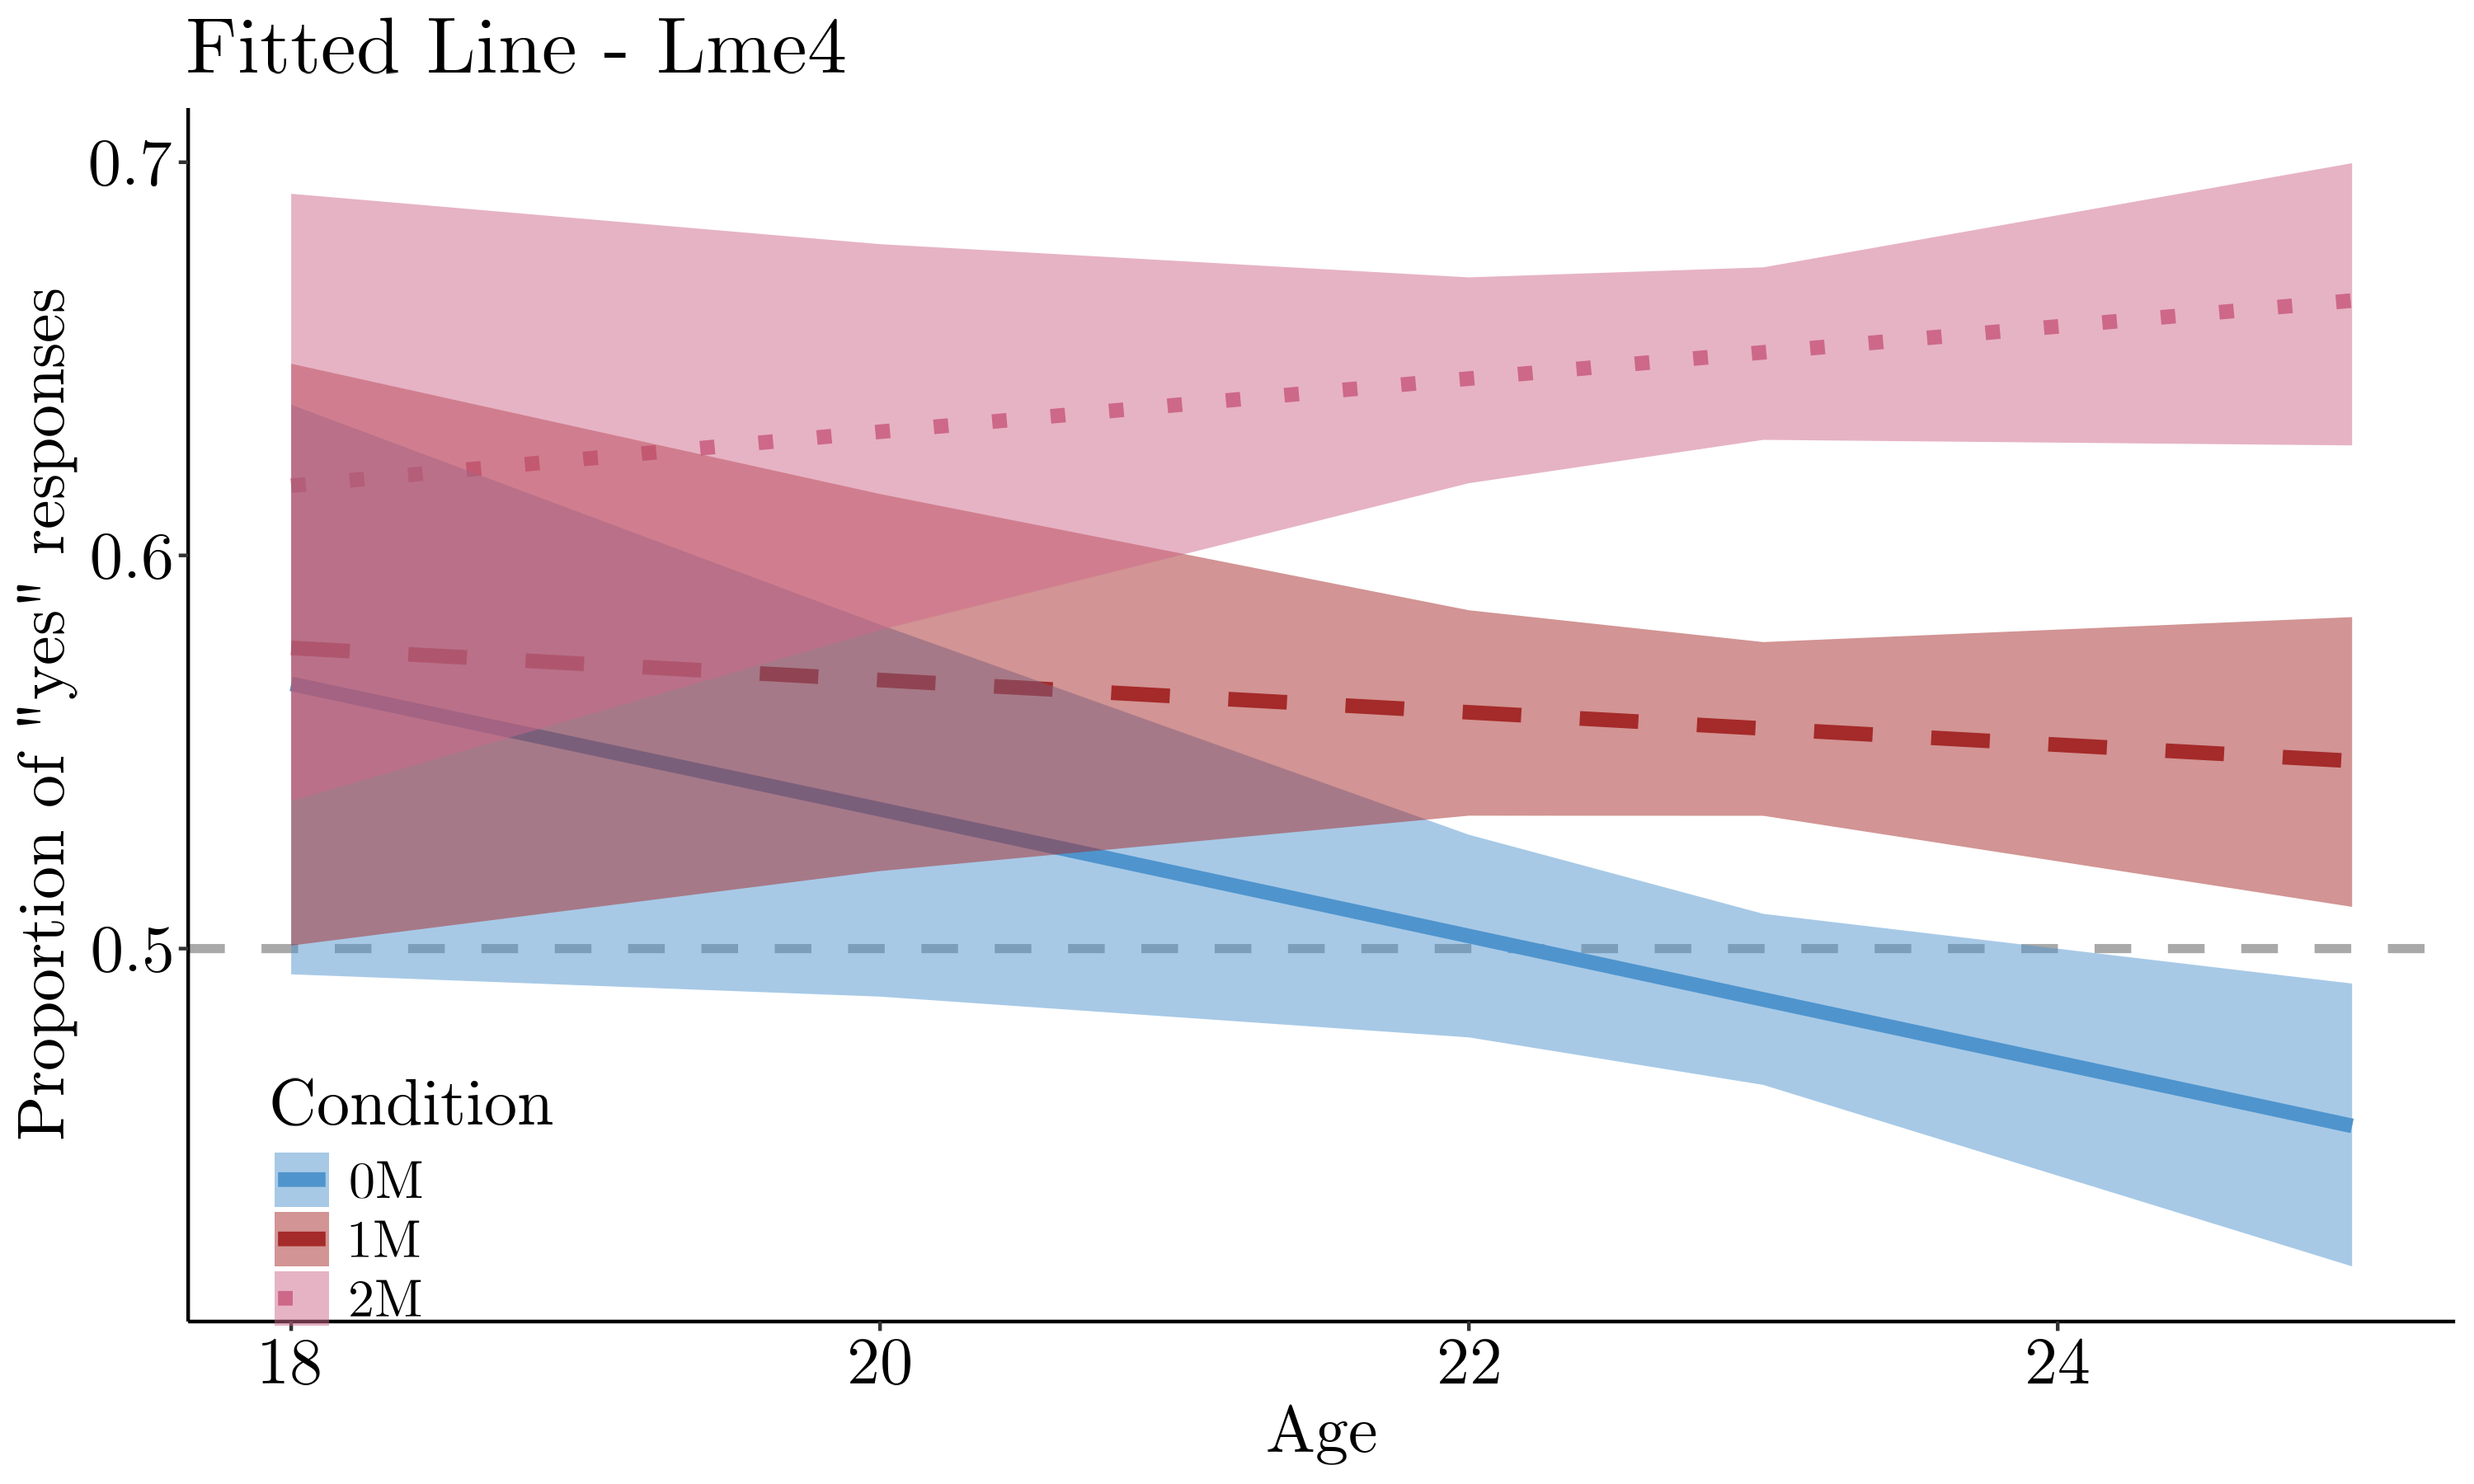
\includegraphics[width=0.99\textwidth]{Figures/Exp1_yes_age.png}
    \end{minipage}
    \begin{minipage}{0.49\linewidth}
        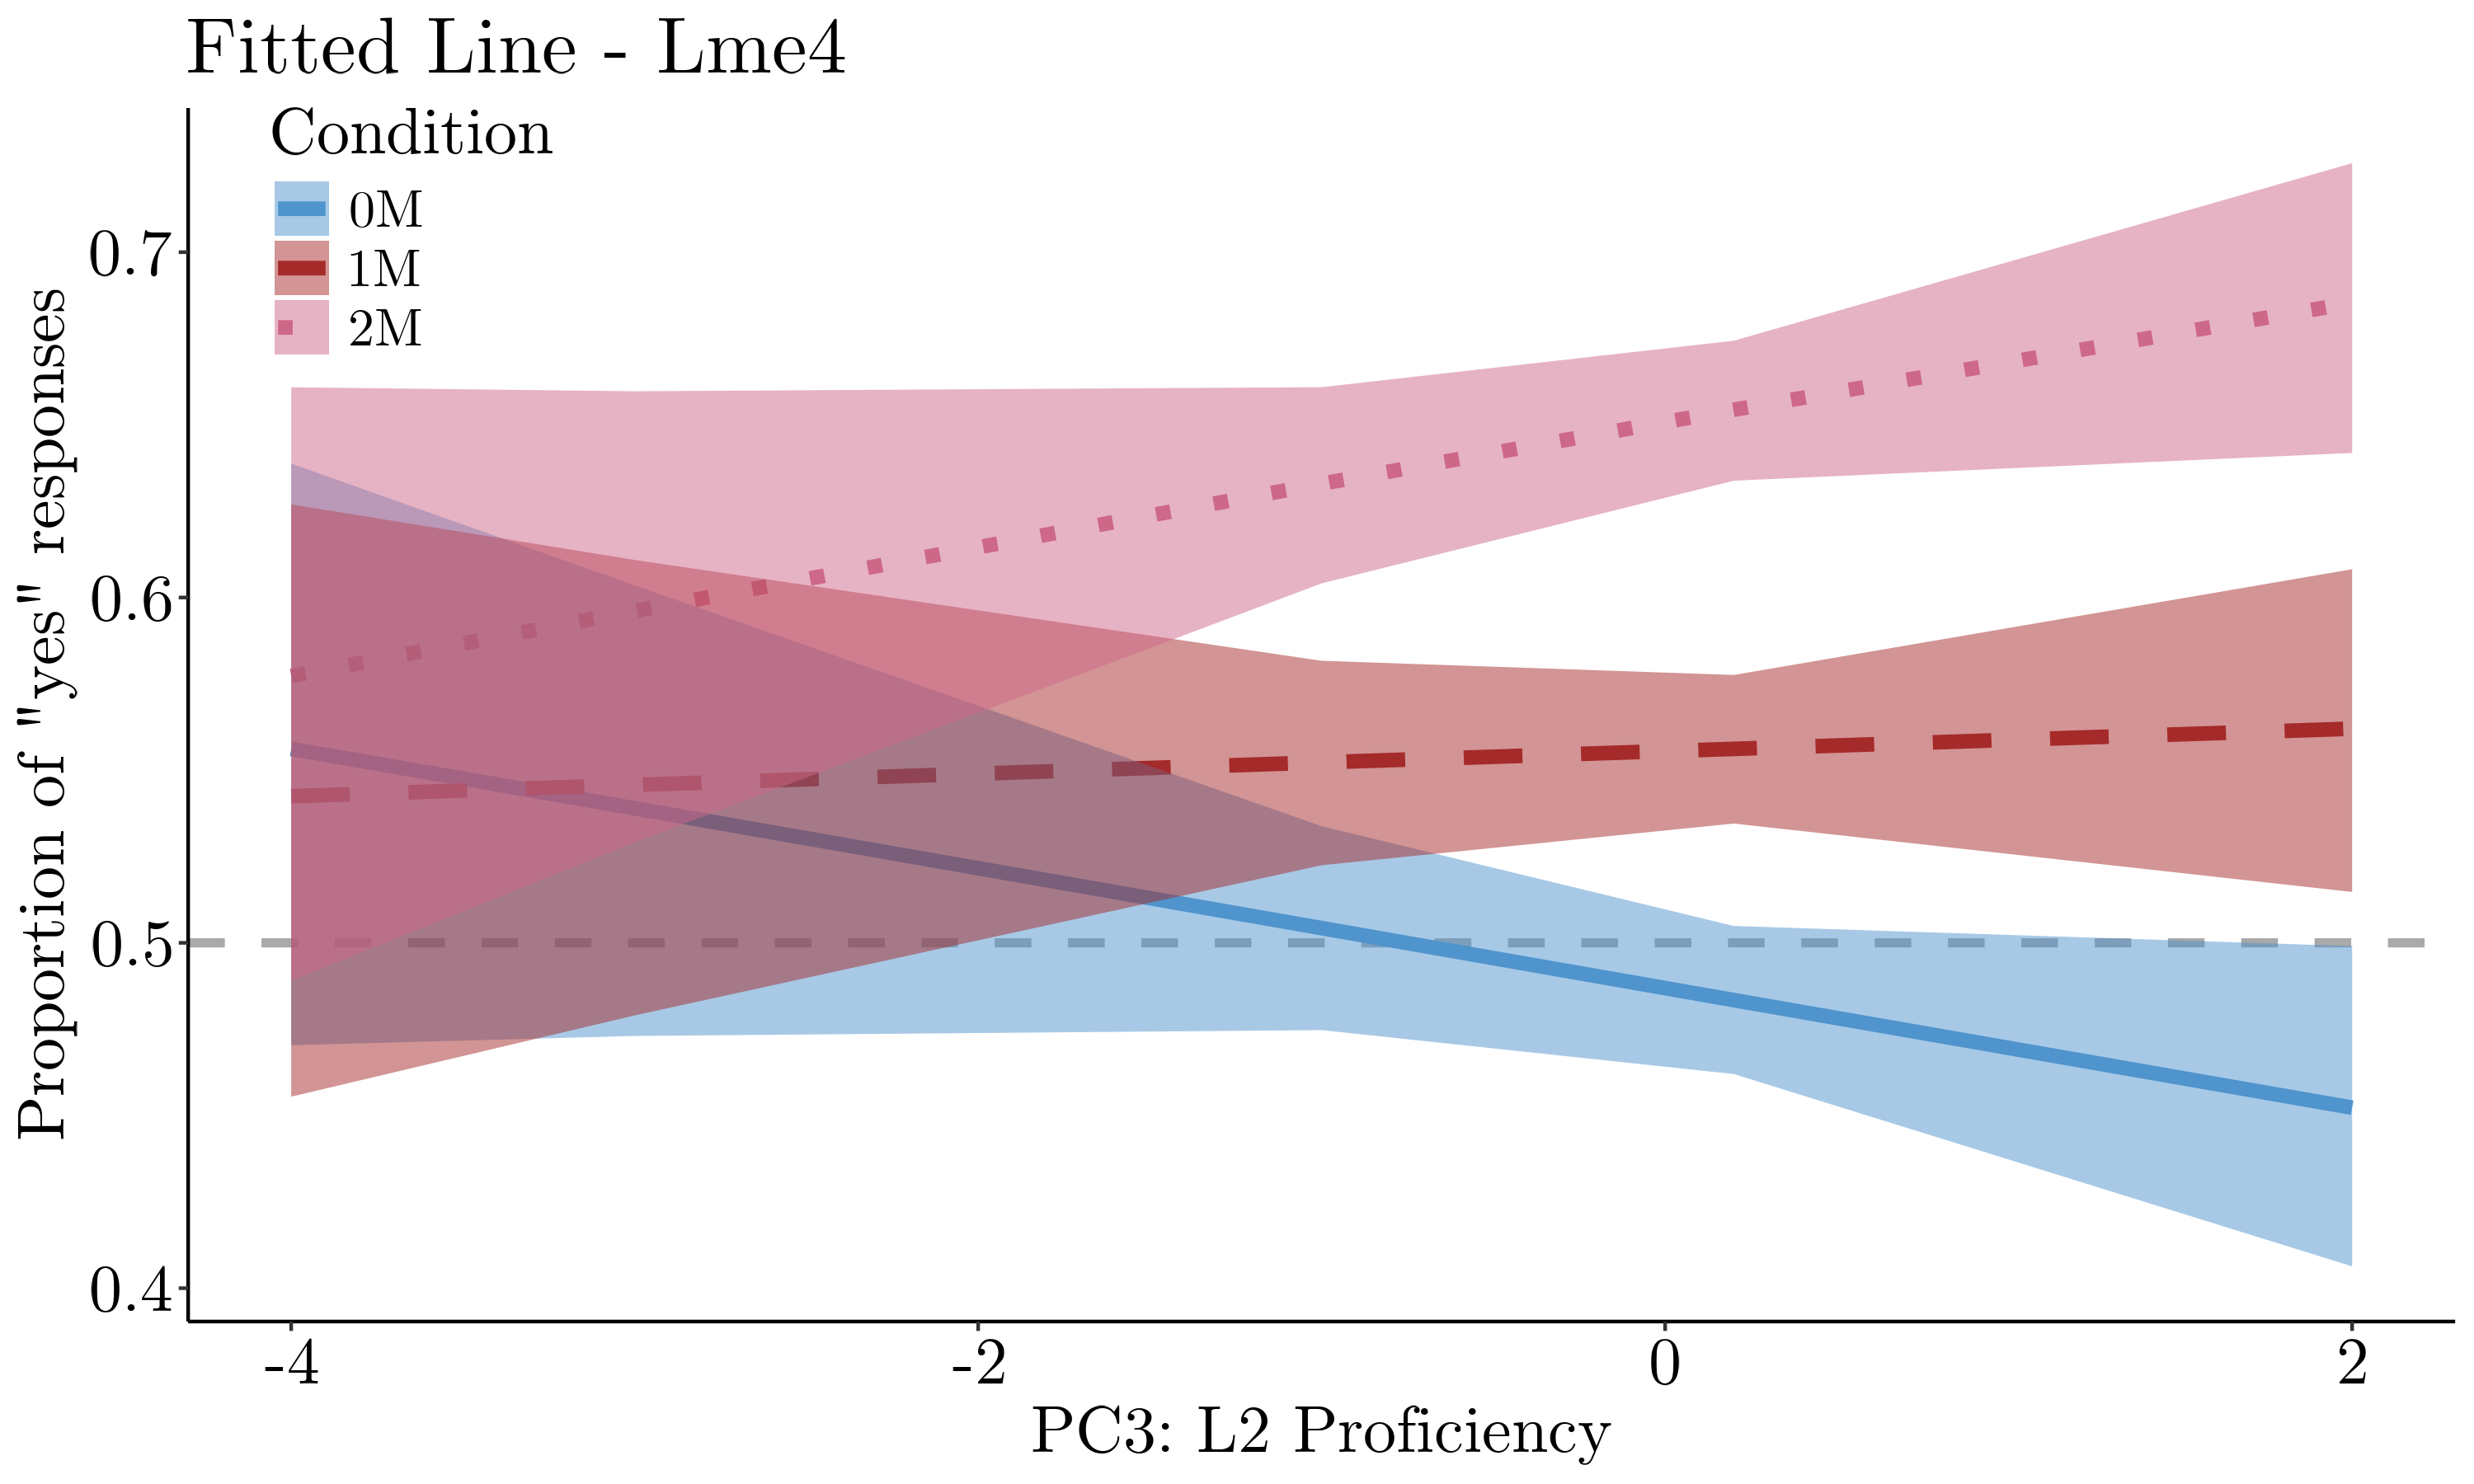
\includegraphics[width=0.99\textwidth]{Figures/Exp1_yes_PC3.png}
    \end{minipage}
    \begin{minipage}{0.49\linewidth}
        \centering
        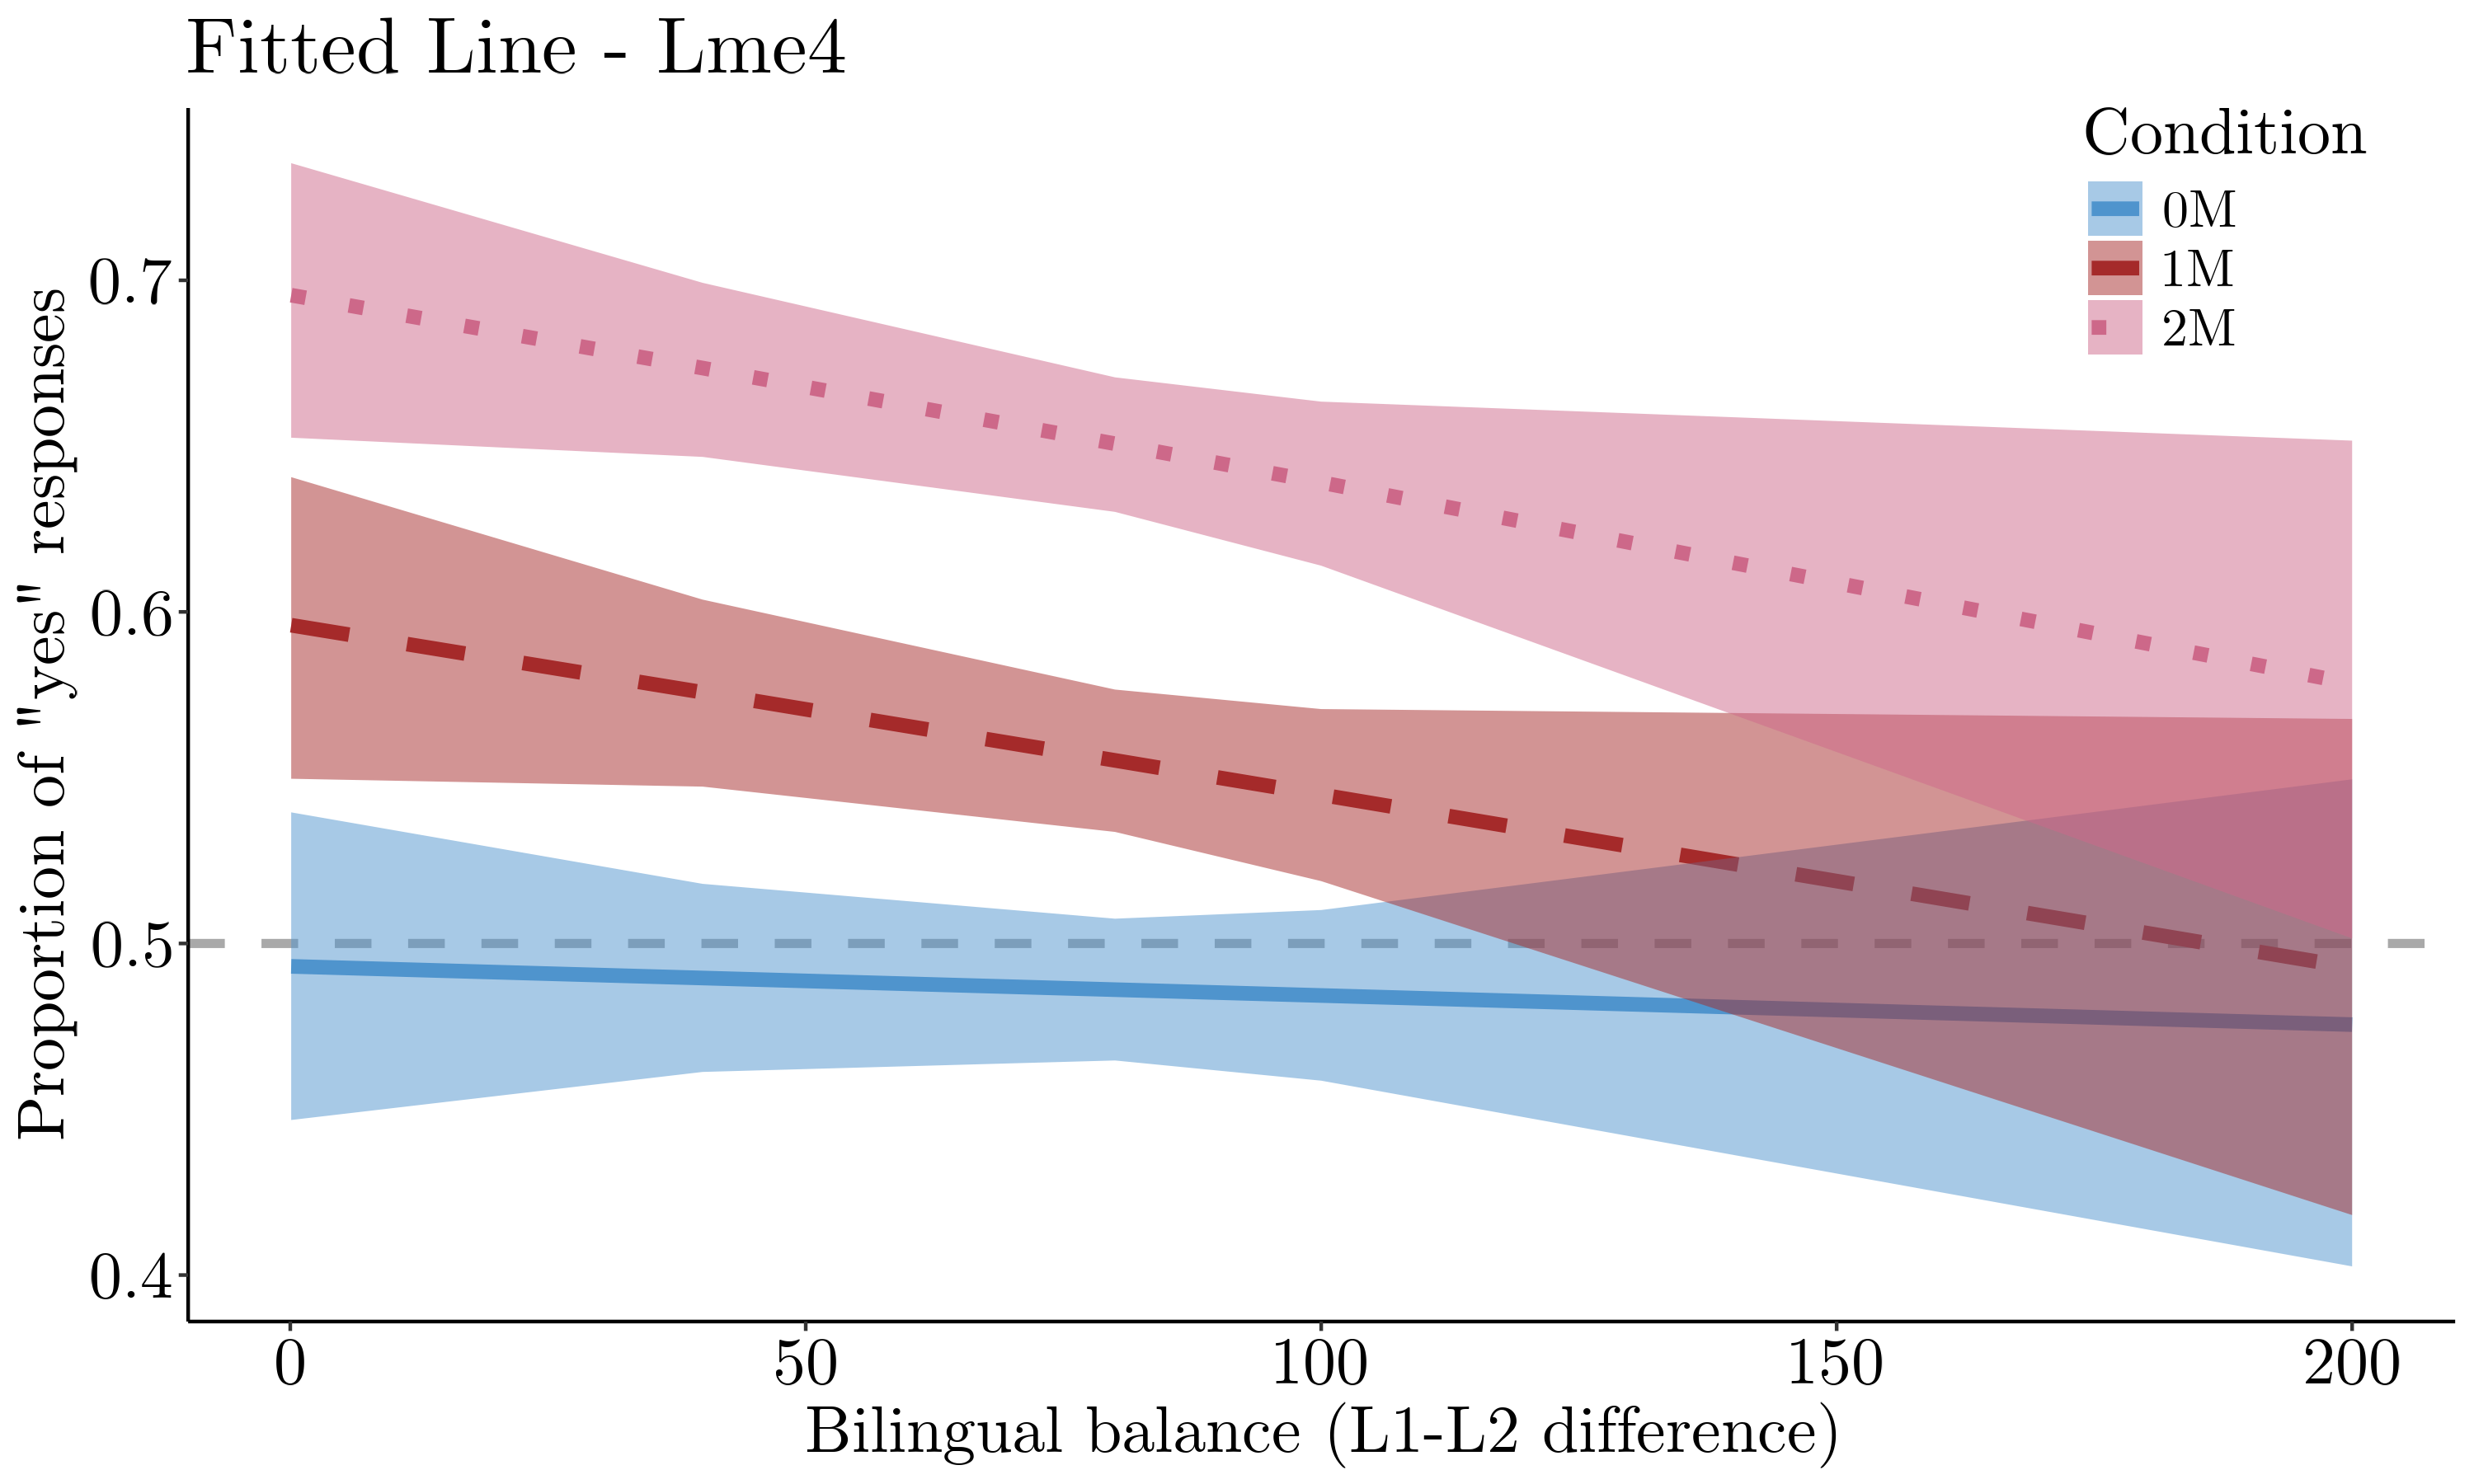
\includegraphics[width=0.99\textwidth]{Figures/Exp1_yes_L1L2diff.png}
    \end{minipage}
    \begin{minipage}{0.49\linewidth}
        \centering
        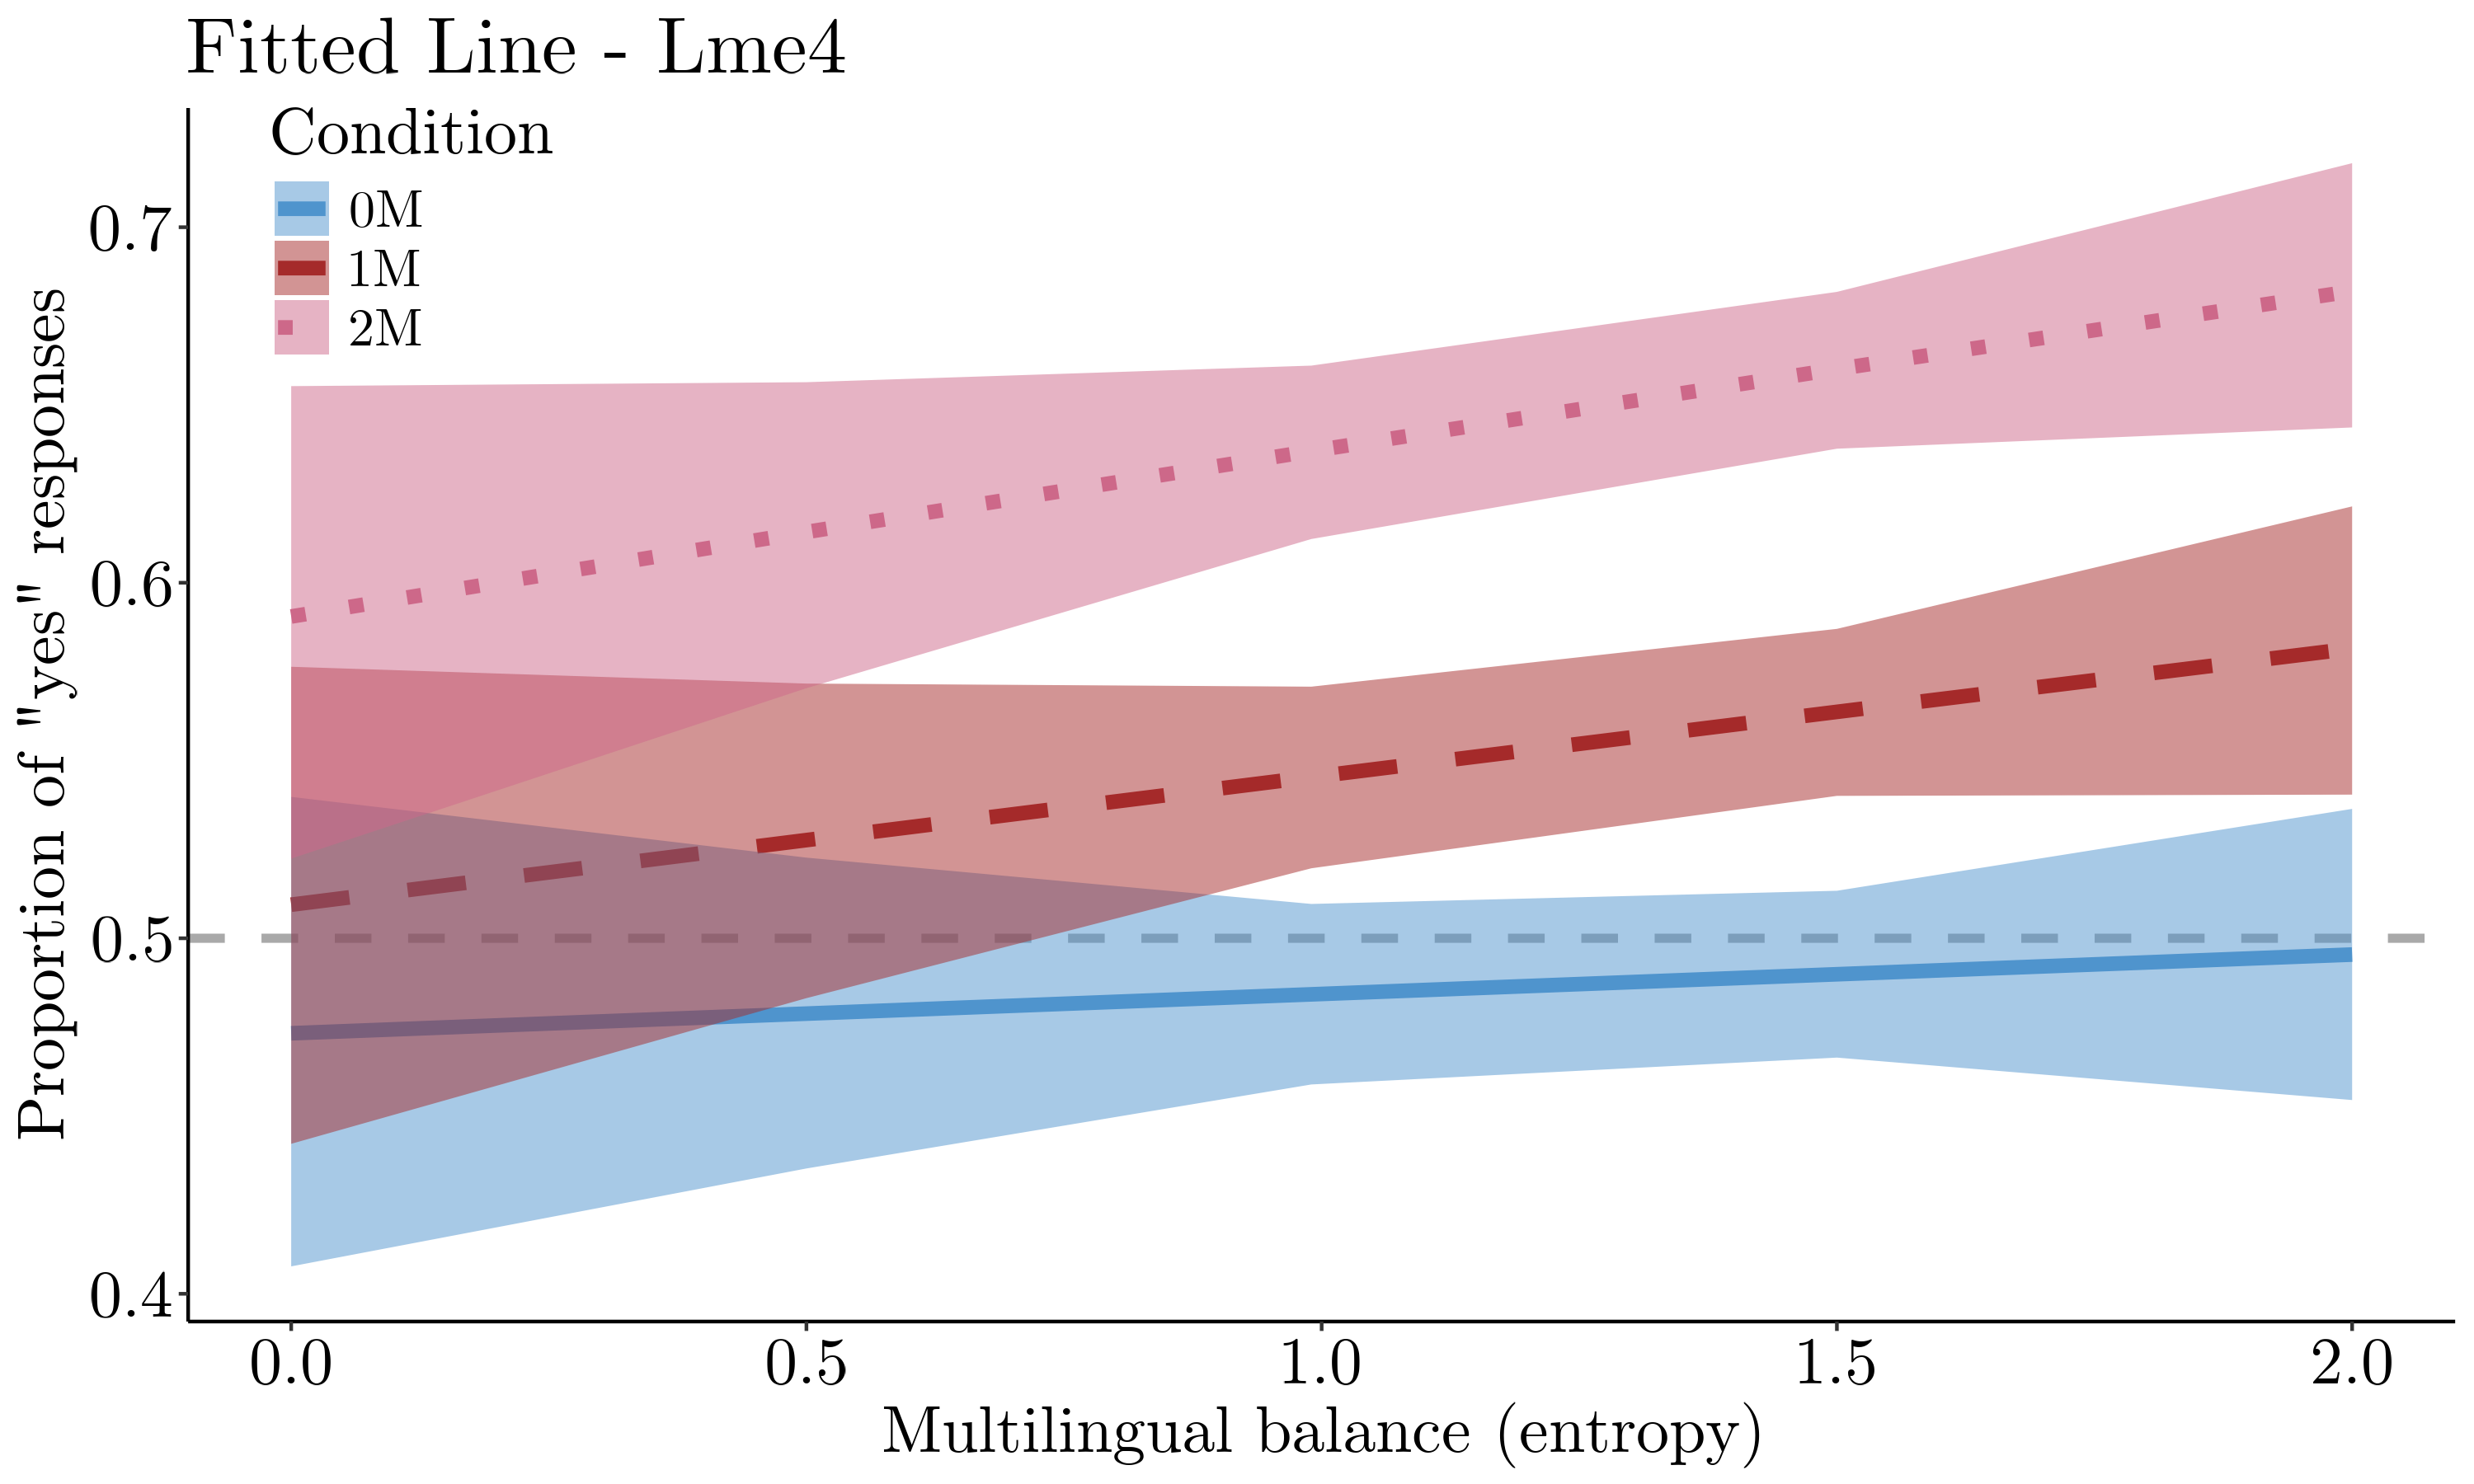
\includegraphics[width=0.99\textwidth]{Figures/Exp1_yes_ent.png}
    \end{minipage}
    \caption[]{\justifying Model estimates of the effect of Age (top left), PC3 (L2 Proficiency; top right), bilingual balance (L1-L2 difference; bottom left), and multilingual balance (entropy; bottom right) on ``yes'' responses, for the 0M (blue), 1M (red), and 2M conditions (pink). Higher values of PC3 entail higher L2 proficiency. L1-L2 difference scores closer to 0 indicate a more balanced bilingual profile, while entropy values closer to 2 indicate a more balanced multilingual profile. Bars around the lines indicate the 95\% confidence interval. Dashed lines at 0.5 indicate chance level.}
    \label{exp1_yes_age/PC3/L1L2diff/ent}
\end{figure}

\begin{table}[!htbp]
    \begin{center}
        \begin{tabular}{@{}lllll@{}}
            \toprule
            \multicolumn{5}{l}{\textbf{``Yes'' responses across conditions}} \\ \midrule
            & \textbf{$\beta$} & \textbf{SE} & \textbf{z-value} & \textbf{p-value} \\ \midrule
            PC8 (L2 history) & 0.11 & 0.04 & 2.38 & 0.02 \\ \midrule
            Age & -0.10 & 0.04 & -2.21 & 0.03 \\ \midrule
            Age$\ast$2M & 0.14 & 0.05 & 2.77 & 0.006 \\ \midrule
            PC3 (L2 proficiency)$\ast$1M & 0.08 & 0.04 & 2.24 & 0.03 \\ \midrule
            PC3 (L2 proficiency)$\ast$2M & 0.15 & 0.05 & 2.91 & 0.004 \\ \midrule
            L1-L2 difference$\ast$1M & -0.10 & 0.04 & -2.81 & 0.005 \\ \midrule
            L1-L2 difference$\ast$2M & -0.13 & 0.04 & -3.65 & 0.0003 \\ \bottomrule
        \end{tabular}
    \end{center}
    \caption{Summary of experiment 1 mixed modelling statistics of ``yes'' responses across conditions, for significant variables.}
    \label{exp1_yes_summary}
\end{table}
\break


\noindent
\underline{2M performance}

\noindent Participant strategies were classified, the most popular of these being the use of one's intuition (declared by 80 participants). The next most used strategies were single letter identification (56 participants) and morpheme identification (25 participants). Given that intuition would rely on participants' implicit knowledge, a Student's t-test was also run on those participants' 2M scores. However, this revealed that their scores were not significantly above chance (t(79) = -0.94, p = 0.35). 

On the other hand, while those using the learned morphemes as a strategy did not have scores significantly above chance (t(24) = 1.01, p = 0.32), they did have a mean d-prime of 0.10. Given that no other variables significantly affected 2M accuracy, this was a good indicator that the task may be too complicated, and only those particularly looking for meaningful chunks in the input were able to successfully detect when they were assembled incorrectly.